% !TEX options=-shell-escape
\documentclass{article}
\usepackage{fancyhdr}
\usepackage{lastpage}
\usepackage{amsthm}
\usepackage{hyperref}
\usepackage{amsmath}
\usepackage{amsfonts}
\usepackage{siunitx}
\usepackage{footnote}
\usepackage{tablefootnote}
\usepackage{makecell}
\usepackage[a4paper, total={5.6in, 8.8in}]{geometry}
\usepackage{longtable}
\usepackage{multirow}
\usepackage{array}
\usepackage{verbatim}
\usepackage{unicode-math}
\usepackage{minted}
\usepackage{booktabs}
\usepackage{algorithm}
\usepackage{algpseudocode}
\usepackage{subcaption}
\usepackage{graphicx}
\usepackage{tocbibind}
\usepackage[toc,page]{appendix}

\setmathfont{XITS Math}

\DeclareMathOperator*{\argmax}{arg\,max}
\DeclareMathOperator*{\argmin}{arg\,min}
\DeclareMathOperator*{\var}{Var}

\setminted{breaklines,tabsize=2}

\newtheorem{assumption}{Assumption}
\newtheorem{definition}{Definition}

\pagestyle{fancy}
\fancyhf{}
\rhead{Page \thepage\ of \pageref{LastPage}}
\lhead{Team \# 10751}

\begin{document}

\begin{center}
Team Control Number

\Huge 10751

\normalsize ~

Problem Chosen

\Huge B

\Large 2020

HiMCM

Summary Sheet
\end{center}

\normalsize

Helping Florida to use the funds in an effective and balanced way is a problem related to the optimization with multiple constraints.
To solve the difficult problem, we developed a knapsack model and a scheduling model to analyze the properties of the projects involved in the conservation plan and find out what mathematical process we are going to go through to reach our goal.
We also modified the algorithm for knapsack problem to solve the model and derive the result: the best schedule of the plan.

We have given formal analysis over all the concepts related to our model,
including the raw attributes of the projects given in the attachments of the problem
and the derived attributes of the plan and projects calculated from the raw attributes.
After analyzing the factors we need to consider for the problem, we find that the problem can be reduced into two smaller problems: a knapsack problem and a scheduling problem.

The knapsack problem is to select proper projects so that the efficiency of the plan is maximized.
We have used a modified algorithm for knapsack problem to solve the knapsack model.
After this step, we have derived the best choice of projects.

The scheduling problem is to decide the start time for the projects in the plan so that the funds spent over time is most balanced.
We have used mathematics to reduce the problem into a minimization of sum of square, and used a rather brute force algorithm to get the result.
This gives us the final schedule of the conservation plan.

Finally, we reviewed our model and listed its pros and cons.
Although some of the general assumptions of the model make its application limited,
the comprehensiveness and effectiveness of our model is significant.

\newpage

\tableofcontents

\newpage
\section{Introduction}
\label{sec:intro}

It is a global issue that the decrease in biodiversity due to the extinction of endangered plants is a serious problem for the balance of the ecosystem.
To avoid this, people need to spend money on protecting the plants and animals.

However, in some places like Florida, greatly needing biodiversity conservation,
people do not have enough money to protect all of the imperiled species there.
They need to find out a proper scheme of funding and protecting to make full use of the funds to get as much benefit as possible.

Different projects of conservation have different cost, benefit, and required time,
as shown in the table of threatened plants data (abbreviated as TPD in the following parts of the paper).
It is to be determined which projects are selected in the optimal plan according to these factors.
After choosing the projects, when to start the projects should also be determined to balance the funds spent over time as possible.

To make it clear what is going to be done, the problem is restated in Section \ref{sec:restatement}.
The model used in our solution to the problem and its explanation are shown in Section \ref{sec:model}.
The algorithms used to solve the model are introduced and explained in Section \ref{sec:approach}.
We will also write a non-technical memo in Section \ref{sec:memo} to give our proposal according to the result of our model.

\section{Restatement and analysis of the problem}
\label{sec:restatement}

Various plant conservation projects with different budgets and timelines are to be conducted.
However, one major issue is that funds are not sufficient to support all projects.
Therefore, it is essential to make a plan for the managers who monitor the whole plan to help them precisely decide which project should be included and when and how to allocate their fund.

What is notable is that the final goal of this plan is not to simply save as many as plant species as possible.
Instead, it should generate greatest benefit meanwhile taking account of different factors, like feasibility of success and the uniqueness of this species.
The time spanning to finish the whole plan is also a factor that needs to be seriously considered because as more time being taken to protect one species, the likelihood of another plant dying out shall increase, finally leading to less benefit.
Another factor is the funds spent on these projects.
Obviously, a project with median benefit but high expense does not fit.
The most suitable plan we need to find out should include all variables mentioned and give the best result.

The mathematical description of the problem is given in Section \ref{sec:model}.
To be specific, the problem is to reach the goal described in Section \ref{sec:goal}.

The factors that we need to consider are
\begin{itemize}
\item The total benefit of the plan should be larger as possible;
\item The time spent on the plan should be shorter as possible;
\item Considering the taxonomic uniqueness of protected species, the benefit of a project may not be fully exerted;
\item Considering the feasibility of success, a project may not be successfully executed;
\item The funds spent over time should be balanced as possible.
\end{itemize}

These factors are coupled in different ways and have different priorities.
Therefore, our work is going to consist of
\begin{enumerate}
\item Giving the mathematical definition and explaining the factors above and related concepts,
\item Analyzing the factors and deriving the way that they are coupled together,
\item Determining the priorities of the factors and thus determining the goals of our mathematical model,
\item Developing algorithms to solve the model and thus reaching the determined goals.
\end{enumerate}

The whole process is mainly shown in Section \ref{sec:model}, explaining the mathematical model, and in Section \ref{sec:approach}, explaining the algorithms.

\section{List of symbols}

To make our model concise and straight forward, a list of symbols are defined as following, as shown in Table \ref{tab:symbols}.
The meaning of the symbols are to be explained in detail in the rest of this article.
In the table, the symbols in lower case are variables w.r.t. a project,
and the symbols in upper case are variables w.r.t. the plan.
The difference between a project and the plan is described in Section \ref{sec:projects and the plan}.

Note that in this article, all numberings
(like $x$ here numbering the projects, and $n$ later numbering the years)
start with $0$ instead of $1$ to meet the convention in computer science.

The symbol $\sum_j^n$ means to sum for $j=0,1,\dots,n-1$.
Similar notations are used for other operators like $\prod$, $\var$ (variance), and so on.

If $X$ is a variable related to the plan, $X^*$ denotes the actual value of the variable in the final optimal plan.

%\begin{definition}[efficiency]
%	The \textbf{efficiency} of a plan is defined as
%	\begin{equation}
%		...
%	\end{equation}
%\end{definition}
%表格
\begin{table}[h!]
\caption{List of symbols}
\label{tab:symbols}
\centering
\begin{tabular}{cccc}
\toprule
Symbol & Domain & Unit & Meaning\\
\midrule
$x$ & $\mathbb N$ & & The index of projects\\
$D$ & $\mathbb N$ & year & Duration of the plan\\
$d_x$ & $\mathbb N$ & year & Duration of project $x$\\
$n$ & $\mathbb N$ & year & Time (index of years)\\
$Z$ & $\mathscr P\left(\mathbb N\right)$ & & The set of chosen projects\\
$F$ & $\left[0,+\infty\right)$ & dollar & Total funds\\
$b_x$ & $\left[0,+\infty\right)$ & osu\tablefootnote{
   The unit osu is invented to represent the unit of benefit.
} & Benefit of project $x$\\
$u_x$ & $\left[0,1\right]$ & & Taxonomic uniqueness of project $x$\\
$s_x$ & $\left[0,1\right]$ & & Feasibility of success of project $x$\\
$c_{x,n}$ & $\left[0,+\infty\right)$ & dollar & Cost of project $x$ in the $n$th year\\
$c_x$ & $\left[0,+\infty\right)$ & dollar/year & Total cost of project $x$\\
$C_n$ & $\left[0,+\infty\right)$ & dollar/year & Cost of the plan in the $n$th year\\
$C$ & $\left[0,+\infty\right)$ & dollar & Cost of the plan\\
$\beta_x$ & $\left[0,+\infty\right)$ & osu & Effective benefit of project $x$\\
$B$ & $\left[0,+\infty\right)$ & osu & Total effective benefit of the plan\\
$T$ & $\left[0,+\infty\right)$ & osu/year & Time efficiency of the plan\\
$\xi$ & $\mathbb N$ & & The longest project in the plan\\
$a_x$ & $\mathbb N$ & year & When project $x$ starts\\
\bottomrule
\end{tabular}
\end{table}

\section{General assumptions}
\label{sec:assumptions}

\begin{assumption}
\label{as:funds at one time}
The funds $F$ are provided off at one time.
\end{assumption}

We do consider the situation that different funds are raised in different years,
but when adjusting $a_x$ in the plan, not when deciding $Z$.
This can simplify the constraint given by the limitation of funds.

If we consider that the funds may be given differently in different years at the first place as a constraint for our plan,
Equation \ref{eq:constraint} will be written in a far more complicated way, which invalidates all the algorithms and theorems stated in Section \ref{sec:approach}.
In fact, without this assumption, the problem becomes NP-hard because it can be reduced to a multi-dimensional knapsack problem \cite{2dknapsacknp}.

This assumption together with Assumption \ref{as:time efficiency over balancing} gives the priority of optimization.

\begin{assumption}
\label{as:no pause}
A project cannot be paused.
\end{assumption}

In this way, the funds spent each year can only be adjusted by adjusting the start time for each project,
but cannot be adjusted by pausing some certain projects.
In other words, it is impossible that the plan requires to pause a project because funds are used up.
This makes it possible that the funds spent by a project during a plan can be described according to only a single number $a_x$.

This assumption also avoids the possibility that a project fails midway when executed, creating better choices for the rest of the plan for remediation.

\begin{assumption}
\label{as:no interrelationship}
Different projects can be executed simultaneously and do not affect each other.
\end{assumption}

We do not consider that different projects may have some actions in common and share their cost, or one project benefit another project and make more total benefit.
Such situations can make the problem extremely hard because the benefits and costs of the projects are coupled in a nonlinear way instead of simplify summed up.

This assumption is used when defining $B$ in Section \ref{sec:effective benefit} because it can only be defined as Equation \ref{eq:total effective benefit} when there are no interrelationships between projects.
It is also used when defining $C_n$ in Section \ref{sec:variance of yearly costs} because it can only be defined as Equation \ref{eq:yearly cost} if there are no interrelationships between projects.

\begin{comment}
\begin{assumption}
	Extra funds' last year can be saved for this year.
	
\end{assumption}
\end{comment}

\begin{assumption}
The plan should not change when it is ongoing.
\end{assumption}

This assumption is necessary to make our result a simple schedule instead of a complicated flow chart.

\begin{assumption}
\label{as:time efficiency over balancing}
The maximization of $T$ is prior to the balancing of funds spent over time (minimizing $\var_n^DC_n$).
\end{assumption}

This assumption together with Assumption \ref{as:funds at one time} plays an important role when describing our final goal of the model in Section \ref{sec:goal}.

\section{The model}
\label{sec:model}

\begin{comment}
\subsection{Relationship of different variable}
Suppose the funds raised each year is a constant $\alpha$, and the total fund raised $\sigma$ is given. Then $\sigma$ can be expressed in terms of $\alpha$:\\
\begin{equation}
	\label{eq:total_fund}
	\sigma=\sum_{u=1}^I\alpha=I\alpha
\end{equation}
\begin{equation}
\alpha=\frac{\sigma}{I}
\label{eq:funds_raised_each_year}
\end{equation}
The total cost of a single project $x$ and $e_x$ can be expressed as:\\
\begin{equation}
e_x=\sum_{v=1}^{T_x}E_x^{v},(x\in{Q_i}\subset \mathbb Z)
\end{equation}
We also can get the total cost of the whole plan:\\
\begin{equation}
\mathbb E=\sum_x e_x,(x\in{Q_i}\subset \mathbb Z)
\end{equation}
From $(3)$, replace $e_x$ with $\sum\nolimits_{n=1}^NE_x^{v}$\\
\begin{equation}
\mathbb E = \sum_x{\sum_{v=1}^{T_x}E_x^{v}},(x\in{Q_i}\subset \mathbb Z)
\end{equation}

\subsection{Evaluation of various project}
The effective benefit of a certain project $x$, $\beta_x$ can be expressed as
\begin{equation}
\beta_x={B_x}\cdot{U_x}\cdot{S_x}
\end{equation}

\par We use effective benefit $\beta_x$ instead of the benefit provided in the table of Threatened Plants Data (TPD) because benefit in the TPD ignores the fact that it relies on the uniqueness of the plant species and feasibility of success. If $U_x$ equals to $0$ (there are lots of other plant species can fill in its position), there is no need to preserve it as the benefit can completely brought by other plant species. Likewise, if $S_x$ equals to $0$ (no probability to succeed at all), even highest benefit remains useless. However, in terms of $\beta_x$ expression, it becomes 0 when $U_x$ or $S_x$ or both equal to 0, indicating no need for protecting this kind of plant.
\par As can be seen in the TPD, both $U_x$ and $S_x$  are in the interval $[0,1]$. When either or both of these variables get close to $1$ (high probability and uniqueness), the benefit $B_x$ of a certain project can be fully displayed:\\
\begin{equation}
\beta_x={B_x} \cdot {U_x} \cdot {S_x} \approx {B_x} \cdot 1 \cdot 1={B_x}
\end{equation}
\par Whether a plan is successful not only depends on how many species it saves or benefit it brings, but also relies on the expense and time spanning to finish it. Another variable $\zeta$ needs to be determined to further evaluate the plan. It can be expressed as:
\begin{equation}
\zeta=\frac{\sum_x ({B_x} \cdot {U_x} \cdot {S_x})}{\mathbb E \cdot I}(x\in{Q_i}\subset \mathbb Z)
\end{equation}
\par By using formula $(4)$, we can further expand it:
\begin{equation}
\zeta=\frac{\sum_x ({B_x} \cdot {U_x} \cdot {S_x})}{(\sum_x e_x) \cdot I}=\frac{\sum_x ({B_x} \cdot {U_x} \cdot {S_x})}{\sum_x {\sum_{v=1}^{T_x}E_x^{v}}\cdot I},(x\in{Q_i}\subset \mathbb Z)
\end{equation}
\par This equation is related to the time and the cost.
When the total cost or the time span is too large, the denominator $e_x \cdot T_x$ would decrease significantly, making $\zeta$ a small figure.
Lower number indicates less efficiency.
$\zeta$ of the optimal plans would be greater than those of other plans.

\subsection{Function and constraint}
\par In the first year, the total fund $F_1$ after fundraising is:
\begin{equation}
F_1=k+\alpha
\end{equation}
Suppose the all the projects that would be conducted in the first year $A_1$ is given, their total cost in the first year can be expressed as:
\begin{equation}
C_1=\sum_{u_1}{E_{u_1}^1},(u_1 \in A_1)
\end{equation}

The total cost in the first year could not exceed the total fund raised. This constraint can be showed as:
\begin{equation}
F_1=k+\alpha > C_1 =\sum_{u_1}{E_{u_1}^1},(u_1 \in A_1)
\end{equation}

\par And the left fund $L_1$ is:
\begin{equation}
L_1=F_1-C_1=k+a-\sum_{u_1} E_{u_1}^1,(u_1 \in A_1)
\end{equation}
\par Second year’s fund is the combination of the fund left in the first year and the fund raised in the second year:
\begin{equation}
F_2=L_1+\alpha
\end{equation}
\par Suppose all projects initiated in the second year $A_2$ is also given, the total cost in the second year $C_2$ the combination of the cost of projects initiated in the first year and projects initiated in the second year:
\begin{equation}
C_2=\sum_{u_1} E_{u_1}^2+\sum_{u_2} E_{u_2}^1,(u_1\in A_1,u_2\in A_2)
\end{equation}
\par Also, the constraint is that the total fund in second year is greater than the total cost:
\begin{equation}
F_2=L_1+\alpha>C_2x```
\end{equation}
\par The fund left in the second year $L_2$ is:
\begin{equation}
L_2=F_2-C_2=L_1+\alpha-C_2=k+2\alpha-(\sum_{u_1} E_{u_1}^2+\sum_{u_2} E_{u_2}^1),(u_1\in A_1,u_2\in A_2)
\end{equation}
\par Based on the same principal, we can find the total cost of projects in $n^{th}$ year:
\begin{equation}
C_n=\sum_{u_1} E_{u_1}^{n}+\sum_{u_2} E_{u_2}^{n-1}+\cdots+\sum_{u_n} E_{u_n}^1=\sum_{i=1}^n {\sum_{u_i} E_{u_i}^{n-i+1}}
\end{equation}
$$(define \forall n-i+1>T_{u_i}:E_ui^{n-i+1}=0)$$
where $(u_p\in A_p,(p=1,2,\cdots,n))$.
And the total fund in $F_n$ can also be found:\\
\begin{equation}
	F_n=L_{n-1}+\alpha=F_{n-1}-C_{n-1}+\alpha=F_{n-1}-\sum_{i=1}^{n-1}\sum_{u_i} E_{u_i}^{(n-1)-i+1}+\alpha
\end{equation}

$$(u_p \in A_p,(p=1,2,\cdots,n-1))$$

Through this recursion formula, we can find $F_n$ in terms of $F_1$:

\begin{equation}
\begin{split}
	F_n&=F_{n-2}-\sum_{i=1}^{n-2} \sum_{u_i} E_{u_i}^{(n-2)-i+1}-\sum_{i=1}^{n-1} \sum_{u_i} E_{u_i}^{(n-1)-i+1}+\alpha+\alpha=F_{n-3}-\cdots+3\alpha\\
	&=F_1-\sum_{j=1}^{n-1} \sum_{i=1}^{j}\sum_{u_i} E_{u_i}^{j-i+1}+(n-1)\alpha=k+\sum_{j=1}^{n-1} {\sum_{i=1}^{j} \sum_{u_i} E_{u_i}^{j-i+1}+n\alpha},
\end{split}
\end{equation}
where $u_p \in A_p$, and $p=1,2,\cdots,n-1)$.

Therefore, by using $(1)$, we can get a series of constraints:

$$F_P>C_p,(p=1,2,\cdots,n)$$
\begin{equation}
k+\sum_{j=1}^{p-1} {\sum_{i=1}^j}{\sum_{u_i}}E_{u_i}^{p-i+1}+p\alpha>\sum_{i=1}^p {\sum_{u_i} E_{u_i}^{p-i+1}},(p=1,2,\cdots,n)
\end{equation}
\begin{equation}
k+\sum_{j=1}^{p-1} {\sum_{i=1}^j}{\sum_{u_i}}E_{u_i}^{p-i+1}+p\frac{\sigma}{I}>\sum_{i=1}^p {\sum_{u_i} E_{u_i}^{p-i+1}},(p=1,2,\cdots,n)
\end{equation}

\par Under these constraints, in order to give the best plan for plant conservation, we need to find the greatest value of $\zeta$ $(9)$:
\begin{equation}
	\zeta = \frac{\sum_x (B_x \cdot U_x \cdot _{S_x})}{(\sum_x \sum_{v=1}^{T_x})\cdot I},(x \in {Q_i} \subset Z=\bigcup\limits_{t=1}^{n} A_t)
\end{equation}
\end{comment}

\subsection{Projects and the plan}
\label{sec:projects and the plan}

The word \textbf{project} is used to represent a conservation of a certain species of plant.
According to the TPD, there are some \textbf{raw data} attributed to a project $x$, which are
the \textbf{unique id}, the \textbf{taxonomic uniqueness} $u_x$, the \textbf{feasibility of success} $s_x$, the \textbf{cost} $c_{x,n}$ of the $n$th year.
These concepts are explained in Section \ref{sec:raw attributes}.

The word \textbf{plan} is used to represent how the projects are going to be executed,
including which projects are executed (the set $Z$) and when they should start (the sequence $\left\{a_x\right\}$).
Deciding the which projects to be executed is to maximize the time efficiency (described in Section \ref{sec:time efficiency}).
Deciding when the projects start is to minimize the variance of yearly cost (described in Section \ref{sec:variance of yearly costs}).

\subsection{Raw attributes of projects}
\label{sec:raw attributes}

To make the concepts more clear and make it easy to use them later,
although the meanings of the raw data are described in the TPD,
their meanings should be re-described in a mathematical way.

\begin{definition}[benefit]
The \textbf{benefit} of project $x$ is a real number $b_x\in\left[0,+\infty\right)$.
\end{definition}

The benefit is an important indicator indicating how imperiled the species is and how easy the project can be done.
However, $b_x$ cannot be directly used to measure how much can we benefit from finishing the project.
Another derived concept called \textbf{effective benefit} should be used instead, as explained in Section \ref{sec:effective benefit}.

\begin{definition}[taxonomic uniqueness]
The \textbf{taxonomic uniqueness} of project $x$ is a real number $u_x\in\left[0,1\right]$.
\end{definition}

The taxonomic uniqueness is a measure of how the species is unique from other species.
It is stipulated that $u_x=0$ if there exists a species that is exactly the same as the species conserved in project $x$,
and $u_x=1$ if the species conserved in project $x$ does not have any similarities with any other species.

\begin{definition}[feasibility of success]
The \textbf{feasibility of success} of project $x$ is a real number $s_x\in\left[0,1\right]$.
\end{definition}

The meaning of $s_x$ is the probability of the success of project $x$.

\begin{definition}[yearly cost]
The \textbf{yearly cost} of project $x$ is a real number $c_{x,n}\in\left[0,+\infty\right)$.
\end{definition}

The meaning of $c_{x,n}$ is cost of project $x$ in the $n$th year.

\subsection{Effective benefit}
\label{sec:effective benefit}

Although $b_x$ is defined for a project, hardly can a project lead to so much benefit finally.
A new concept should be defined to describe how much can people actually benefit from finishing the project.

\begin{definition}[effective benefit]
The \textbf{effective benefit} of a project is a real number $\beta_x\in\left[0,+\infty\right)$ defined as
\begin{equation}
\label{eq:effective benefit}
\beta_x:=b_xu_xs_x.
\end{equation}
\end{definition}

Here is the explanation of why the effective benefit should be defined as Equation \ref{eq:effective benefit}.

First, consider the effect of $u_x$.
If $u_x=0$, which means there is a species the same as the conserved species,
the conservation is useless because even if the conserved species die out, there are other species taking the place.
If $u_x=1$, which means there are no similar species to the conserved species,
the conservation is meaningful and can exert full benefit.
From these two cases, it is reasonable to multiply $b_x$ with $u_x$,
which means $u_x$ represents the portion of $b_x$ that can be exerted if the project is successfully finished.

Then, consider the effect of $s_x$.
It is a probability, so the effect should be considered statistically.
Imagine there are many parallel universes, in each of which project $x$ is carried out under the same condition.
According to the law of large numbers, the portion of successful executions is the probability $s_x$, exerting the benefit,
while the rest does not make any benefit.
Then, the mean of all the benefits is $s_x\cdot b_x+\left(1-s_x\right)\cdot0=b_xs_x$.

Combining the two effects above, the formula for effective benefit (Equation \ref{eq:effective benefit}) can be derived.

From now on, when measuring how much can a project benefit people,
$\beta_x$ is used instead of $b_x$.

By summing up the effective benefit for all projects of the plan, the total effective benefit can be defined.

\begin{definition}[total effective benefit]
The \textbf{total effective benefit} of the project is a real number $B\in\left[0,+\infty\right)$ defined as
\begin{equation}
\label{eq:total effective benefit}
B:=\sum_{x\in Z}b_x.
\end{equation}
\end{definition}

The $B$ is an important indicator of how much a plan is expected to benefit if the plan is executed.

\subsection{Duration}
\label{sec:duration}

The \textbf{duration} of a project is the time for which it lasts.
It can be defined according to the yearly costs of the project.

\begin{definition}[duration of project]
The \textbf{duration of project} $x$ is a real number $d_x\in\mathbb N$ defined as
\begin{equation}
d_x:=\min\left\{m\in\mathbb N\middle|\forall n\ge m:c_{x,n}=0\right\}
\end{equation}
\end{definition}

According to the TPD, a project must be able to end, which means such $d_x$ must exist.

The duration of the plan should be defined as the time interval between the time when the first project of the plan starts and the time when the last project of the plan ends.
However, due to Assumption \ref{as:time efficiency over balancing}, the duration of the plan should unnecessarily be defined in a so straight-forward way.
A better definition is given in Equation \ref{eq:duration of the plan} in Section \ref{sec:time efficiency}.

\subsection{Time efficiency}
\label{sec:time efficiency}

\begin{definition}[time efficiency]
The \textbf{time efficiency} of the plan is a real number $T\in\left[0,+\infty\right)$ defined as
\begin{equation}
T:=\frac BD.
\end{equation}
\end{definition}

The time efficiency of the plan is the average benefit gain during a unit of time.
It should be maximized to make the plan as efficient as possible,
whose reason can be found in Section \ref{sec:goal}.

According to Assumption \ref{as:time efficiency over balancing}, $T$ should be maximized before we think about how $a_x$ can be adjusted to balance the funds spent over time.
To maximize the time efficiency, the duration of the plan is the same as the duration of the project with the largest duration ($\xi$) in the plan,
where $\xi$ is the project with largest duration among $Z$
\begin{equation}
\xi:=\argmax_{x\in Z}d_x.
\end{equation}
Then, when $a_x$ are adjusted to minimize variance of yearly costs,
the start time of projects with shorter duration than $d_\xi$ will never be changed to make them start before $\xi$ starts or end after $\xi$ ends
because otherwise $D$ increases and thus makes $T$ smaller.
Therefore, rather than the straight-forward definition shown in Section \ref{sec:duration}, there is a better definition.

\begin{definition}[duration of the plan]
The \textbf{duration of the plan} is a real number $D\in\mathbb N$ defined as
\begin{equation}
\label{eq:duration of the plan}
D:=\max_{x\in Z}d_x.
\end{equation}
\end{definition}

It is obvious that if $C$ stays the same, the larger $T$ is, the better the plan is.
In fact, maximizing $T$ is of the most priority.
It may be surprising that the most prior goal is not maximizing $\frac TC$, which is more intuitive.
We do not try to maximize $\frac TC$ because if we did that,
it would lead to a trivial result:
the plan only contains one project with the minimum $\frac{\beta_x}{d_xc_x}$, which is not what we want to see.

\begin{proof}
Without loss of generality, assume that there are only $2$ plant candidates for the plan,
and then the mathematical induction can be used to generalize the conclusion to any number of plant candidates.

Without loss of generality, assume that $d_0\le d_1$, which means $D=d_1\ge d_0$.

Case 1: $\frac{\beta_0}{c_0}\le\frac{\beta_1}{c_1}$.

In this case,
\begin{equation*}
\frac{\beta_0}{c_0}\le\frac{\beta_0+\beta_1}{c_0+c_1}\le\frac{\beta_1}{c_1}.
\end{equation*}
Thus, if the plan consists of both the $2$ projects,
\begin{equation*}
\frac TC=\frac{\beta_0+\beta_1}{c_0+c_1}\cdot\frac1{d_1}\le\frac{\beta_1}{c_1d_1}.
\end{equation*}
Therefore, the plan consisting of only project $1$ is better than that of both projects.

Case 2: $\frac{\beta_0}{c_0}>\frac{\beta_1}{c_1}$.

Similarly to case 1, in this case,
\begin{equation*}
\frac{\beta_0}{c_0}>\frac{\beta_0+\beta_1}{c_0+c_1}>\frac{\beta_1}{c_1}.
\end{equation*}
Thus, if the plan consists of both the $2$ projects,
\begin{equation*}
\frac TC=\frac{\beta_0+\beta_1}{c_0+c_1}\cdot\frac1{d_1}<\frac{\beta_0}{c_0d_1}\le\frac{\beta_0}{c_0d_0}.
\end{equation*}
Therefore, the plan consisting of only project $0$ is better than that of both projects.

From the $2$ cases above, it can be derived that there always exists a plan with single project having the largest $\frac TC$ compared to any other plan.
\end{proof}

\subsection{Variance of yearly costs}
\label{sec:variance of yearly costs}

First, yearly costs need defining.
The yearly cost in the $n$th year of the plan is the sum of the costs of the projects in the $n$th year.
It should take into account the different start time of the projects.

\begin{definition}[start time]
The \textbf{start time} of project $x$ is a real number $a_x\in\mathbb N$.
\end{definition}

\begin{definition}[yearly costs]
The \textbf{yearly cost} of the plan in the $n$th year is a real number $C_n\in\left[0,+\infty\right)$ defined as
\begin{equation}
\label{eq:yearly cost}
C_n:=\sum_{x\in Z}c_{x,n-a_x}.
\end{equation}
\end{definition}

To measure how balanced the spent funds are distributed through time, the variance of yearly costs $\var_n^DC_n$ is defined.
In Section \ref{sec:goal}, it is going to be minimized to balance the funds spent over time.

It can be proved that minimizing $\var_n^DC_n$ is the same as minimizing $\sum_n^DC_n^2$.

\begin{proof}
In this proof, symbol ``$\sim$'' denotes that two expressions have the same monotonicity.
\begin{align*}
\var_n^DC_n&=\frac1D\sum_n^D\left(C_n-\frac CD\right)^2\\
&\sim\sum_n^D\left(C_n^2-\frac{2C}DC_n+\frac{C^2}{D^2}\right)\\
&=\sum_n^DC_n^2-\frac{2C}D\sum_n^DC_n+\sum_n^D\frac{C^2}{D^2}\\
&=\sum_n^DC_n^2-\frac{C^2}D\\
&\sim\sum_n^DC_n^2.
\end{align*}
Thus, minimizing $\var_n^DC_n$ is the same as minimizing $\sum_n^DC_n^2$.
\end{proof}

\subsection{Constraints to the plan}
\label{sec:constraints}

First, consider the constraint due to the limitation of funds.
To describe the constraint, the total funds and the cost of the plan needs defining.

\begin{definition}[total funds]
The \textbf{total funds} is a real number $F\in\left[0,+\infty\right)$.
\end{definition}

\begin{definition}[cost of project]
The \textbf{cost of project} is a real number $c_x\in\left[0,+\infty\right)$ defined as
\begin{equation}
c_x:=\sum_n^\infty c_{x,n}.
\end{equation}
\end{definition}

The sum $c_x$ must converge because all terms following the $d_x$th term are $0$.

\begin{definition}[cost of the plan]
The \textbf{cost of the plan} is a real number $C\in\left[0,+\infty\right)$ defined as
\begin{equation}
C:=\sum_{x\in Z}c_x.
\end{equation}
\end{definition}

Due to Assumption \ref{as:funds at one time}, the constraint should be
\begin{equation}
\label{eq:constraint}
C\le F.
\end{equation}

There are also constraints resulting from the restrictions for $a_x$ due to the optimization of $T$.
According to the discussions in Section \ref{sec:time efficiency}, any projects in the plan should not start before the longest project start or end after the longest project end.
Let the start time of the longest project in the plan be the $0$th year, and then we have constraints for the start time.
\begin{equation}
\label{eq:start time constraint}
\forall x\in Z:a_x\in\left[0,D-d_x\right).
\end{equation}

\subsection{The goal of the model}
\label{sec:goal}

The goal of the model is to
\begin{enumerate}
\item Decide proper $Z$ to make the plan have the maximum $T$,
\item Decide the minimum $F$ to satisfy step 1 under the constraint Equation \ref{eq:constraint},
\item Decide the $a_x$ for each chosen project in step 1 to minimize $\var_n^DC_n$ under the constraint Equation \ref{eq:start time constraint}.
\end{enumerate}

In this way, the derived plan can meet the requirements described in Section \ref{sec:restatement}.

To reach the goal, we need to develop some approaches based on the model,
which are described in Section \ref{sec:approach}.

\section{The algorithms}
\label{sec:approach}

In Section \ref{sec:goal}, it is stated that the first step is to maximize $T$ regardless of constraint Equation \ref{eq:constraint}.
However, because it is actually not known whether max $T$ can increase constantly as long as allowable $C$ increase until all projects available is chosen in $Z$.
To study the trend of how max $T$ under constraint Equation \ref{eq:constraint} changes when $F$ increases, the actual step of our approach is to
\begin{enumerate}
\item Develop a program to maximize $B$ given $F$,
\item Develop a program based on the last program to maximize $T$ given $F$,
\item Ensure that $T$ has a maximum value $T^*$ whenever $F\ge F^*$, where $F^*$ is to be determined,
\item Develop a program to minimize $\var_n^DC_n$.
\end{enumerate}

\subsection{Maximize $B$ given $F$ under constraint Equation \ref{eq:constraint}}

This subproblem is a 0-1 knapsack problem, regarding
\begin{itemize}
\item $F$ as the capacity of the knapsack,
\item $c_x$ as the weight of the $x$th item,
\item $\beta_x$ as the value of the $x$th item.
\end{itemize}

There is a classic dynamic programming (DP) algorithm to solve knapsack problems \cite{dpknapsack},
shown in Algorithm \ref{alg:dp}.

\begin{algorithm}[h!]
\caption{Classic DP algorithm for 0-1 knapsack problem}
\label{alg:dp}
\begin{algorithmic}
\State Integerize $F$
\For{each project $x$}
	\State Integerize $c_x$
\EndFor
\Function{knapsack}{$F$}
\State Initialize $m$ as an array whose elements are all $0$
\State Initialize $p$ as an array whose elements are all $\emptyset$
\For{each project $x$}
	\For{$w$ from $F$ down to $c_x$}
		\If{$m\left[w\right]<m\left[w-c_x\right]+\beta_x$}
			\State$m\left[w\right]\leftarrow m\left[w-c_x\right]+\beta_x$
			\State$p\left[w\right]\leftarrow p\left[w-c_x\right]\cup x$
		\EndIf
	\EndFor
\EndFor
\State\Return$m\left[F\right],p\left[F\right]$
\EndFunction
\end{algorithmic}
\end{algorithm}

However, this algorithm does not fit with our problem here
because $F$ and $c_x$ should be natural numbers to appear as index of elements in arrays like $m$ and $p$.
The conflict can be resolved by rounding the values into integers,
but due to the large capacity of the knapsack and the large weight of the items,
the algorithm cannot give a result in acceptable time until the rounding makes the inaccuracy so significant that the result is not convincing at all.

Thus, a new algorithm should be developed.
The main reason for Algorithm \ref{alg:dp} to be slow is that it traverse through a whole continuous part of array $m$ whenever it traverse a project $x$,
while most of the elements in $m$ are useless and are unnecessary to be updated.
However, whether an element in $m$ is useful cannot be determined using the DP algorithm.
Inspired by this thought, the recursive algorithm can be adopted because it can make the program consider small $w$ values first and determine which $w$ values later on are useful.
The new algorithm is shown in Algorithm \ref{alg:recursive}.

\begin{algorithm}[h!]
\caption{Recursive algorithm for 0-1 knapsack problem}
\label{alg:recursive}
\begin{algorithmic}
\Function{recursive}{$F,x$}
\If{$x$ exceeds the limit of projects}
	\State\Return$0,\emptyset$
\ElsIf{$c_x>F$}
	\State\Return$\Call{recursive}{F,x+1}$
\Else
	\State$m_1,p_1\leftarrow\Call{recursive}{F,x+1}$
	\State$m_2,p_2\leftarrow\Call{recursive}{F-c_x,x+1}$
	\If{$m_1<m_2+\beta_x$}
		\State\Return$m_2+\beta_x,p_2\cup x$
	\Else
		\State\Return$m_1,p_1$
	\EndIf
\EndIf
\EndFunction
\Function{knapsack}{$F$}
\State\Return$\Call{recursive}{F,0}$
\EndFunction
\end{algorithmic}
\end{algorithm}

However, when there are many projects, the recursive algorithm even takes more time than the DP algorithm
because there some $\left(F,x\right)$ being calculated multiple times.
Since this recursive function is a pure function, a cache can be used to store previously calculated result.
Nonetheless, since $F$ and $c_x$ are floating numbers, the probability of cache hit is low.
To increase the probability of cache hit, the numbers should be rounded.
In our case, they are rounded to $\SI{100}{dollars}$.

There can also be some other optimizations.
The projects can be sorted according to their costs, so that the condition branch $c_x>F$ can be designed to be a short-circuit evaluation,
immediately returning $0,\emptyset$ because the rest projects are even more expensive.

The optimized version is shown in Algorithm \ref{alg:optimized recursive}.

\begin{algorithm}[h!]
\caption{Recursive algorithm for 0-1 knapsack problem, optimized with cache and short-circuit evaluation}
\label{alg:optimized recursive}
\begin{algorithmic}
\State Integerize $F$
\For{each project $x$}
	\State Integerize $c_x$
\EndFor
\State Sort the projects w.r.t. $c_x$
\Function{recursive}{$F,x$}
\If{$k\left[F,x\right]$ exists}
	\State\Return$k\left[F,x\right]$
\ElsIf{$x$ exceeds the limit of projects \textbf{or} $c_x>F$}
	\State\Return$k\left[F,x\right]\leftarrow0,\emptyset$
\Else
	\State$m_1,p_1\leftarrow\Call{recursive}{F,x+1}$
	\State$m_2,p_2\leftarrow\Call{recursive}{F-c_x,x+1}$
	\If{$m_1<m_2+\beta_x$}
		\State\Return$k\left[F,x\right]\leftarrow m_2+\beta_x,p_2\cup x$
	\Else
		\State\Return$k\left[F,x\right]\leftarrow m_1,p_1$
	\EndIf
\EndIf
\EndFunction
\Function{knapsack}{$F$}
\State Initialize $k$ as a key-value mapping
\State\Return$\Call{recursive}{F,0}$
\EndFunction
\end{algorithmic}
\end{algorithm}

Algorithm \ref{alg:optimized recursive} is implemented in Ruby as part of Appendix \ref{appendix:prog min T}.

\subsection{Maximize $T$ given $F$ under constraint Equation \ref{eq:constraint}}

The plan given by maximizing $B$ may not have maximum $T$.
The only thing that can be ensured is that $T$ cannot increase without reducing $D$.
According to Equation \ref{eq:duration of the plan}, $D$ is determined by the longest project.
Thus, if we want to increase $T$, we need to remove the longest project in the selected plan,
and find another plan that maximizes $B$ without using the project that we have just removed.
The process is cycled until no projects are chosen.

From this insight, the pseudocodes shown in Algorithm \ref{alg:max T funds}.
The algorithm is implemented in Ruby in Appendix \ref{appendix:prog min T}.

\begin{algorithm}[h!]
\caption{Algorithm for maximizing $T$ given $F$}
\label{alg:max T funds}
\begin{algorithmic}
\State$m,p\leftarrow0,\emptyset$
\Loop
	\State$B,Z\leftarrow\Call{knapsack}{F}$
	\If{$Z=\emptyset$}
		\State\Return$m,p$
	\EndIf
	\If{$m<T$}
		\State$m,p\leftarrow T,Z$
	\EndIf
	\State Remove project $\xi$ from the set of all projects
\EndLoop
\end{algorithmic}
\end{algorithm}

After running the program, the curve of max $T$ related to $F$ can be drawn,
as shown in Figure \ref{fig:max T funds}.
As can be seen, although $F$ increases until there are enough funds to execute all the projects simultaneously,
max $T$ does not increase constantly but reaches its maximum when $F\ge F^*$.
It can be derived that $F^*=\SI{11010118.27}{dollars}$ and $T^*=\SI{1638017.60}{osu/year}$.
The chosen plants are shown in Table \ref{tab:schedule} in Section \ref{sec:memo}.

\begin{figure}[h!]
\centering
\begin{subfigure}[b]{\linewidth}
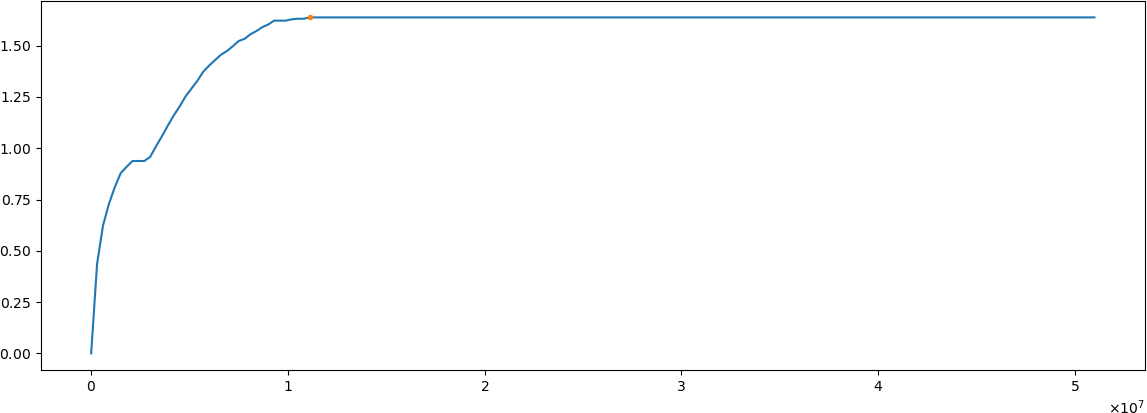
\includegraphics[width=\linewidth]{max_time_efficiency_with_funds.png}
\caption{Overview of the whole graph, where the orange point is $\left(F^*,T^*\right)$}
\end{subfigure}
\begin{subfigure}[b]{0.45\linewidth}
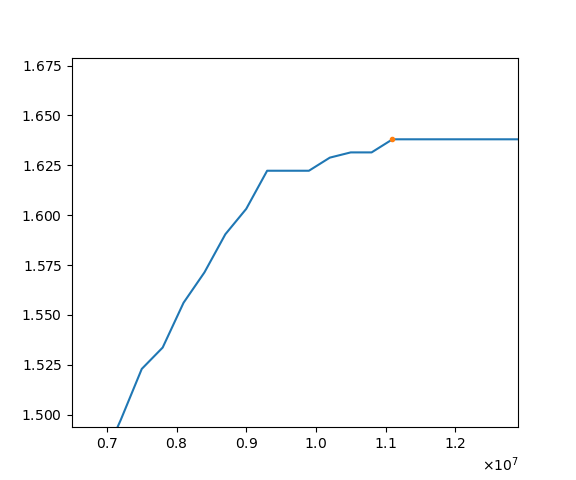
\includegraphics[width=\linewidth]{max_time_efficiency_with_funds_detail.png}
\caption{Details of the graph near $\left(F^*,T^*\right)$}
\end{subfigure}
\caption{The graph of max $T$ related to $F$}
\label{fig:max T funds}
\end{figure}

\subsection{Minimizing \texorpdfstring{$\var_n^DC_n$}{varnDCn} under constraint Equation \ref{eq:start time constraint}}

In Section \ref{sec:variance of yearly costs}, it has been proved that minimizing $\var_n^DC_n$ is the same as minimizing $\sum_n^DC_n^2$,
which can reduce some calculations in calculating the variance (while does not help come up with a smart algorithm because still, the problem is NP-hard).

Here, a brute force algorithm is adopted.
It traverses through all possible start times (as many as $\prod_{x\in Z}\left(D-d_x\right)$ cases).
The algorithm is implemented in Ruby in Appendix \ref{appendix:decide start time}.

After running the program, the optimal $\left\{a_x\right\}$ can be derived.
The optimal $\left\{a_x\right\}$ are shown in Table \ref{tab:schedule} in Section \ref{sec:memo} in form of a schedule.
The minimum value of $\sum_n^DC_n^2$ is $\SI{26457147921183.15}{dollars^2}$.

\begin{comment}
\subsection{Find the maximum effective benefit that can be loaded into the package with given funds}
We turn the question into a question with $n$ items and $a$ backpack with capacity $F$.
The cost of item $x$ is $C[x]$ and the value is $\beta[i]$. 
Find out which items are loaded into the backpack to maximize the total value.
We used the recursive algorithm. Here is our procedure


Firstly, Convert the data in TPD into an array.

Secondly, calculate the value of each item under unit weight $K[x]$ = $\frac{\beta[x]}{C[x]}$, and sort them from large to small according to their value. 
If the they are same, sort them according to their weight.

Thirdly, we set a sequence $ok[x]$ to store whether the corresponding items are loaded or not, 1 means yes, 0 means no.(the initial values are all 0).

Define the function $v = fn(F, POS)$, input: $F$, that is, the current maximum weight that can be carried, and $POS$ refers to the number of positions in the array to calculate.\\
The algorithm of recursive function is shown as follows:\\
1. Judge whether the weight of the object at $POS$ is bigger than in $F$.\\
2. If True, give up the item in the position, and the function returns $fn(F, POS + 1)$. If it is the last one, return 0 directly.\\
3. If Fulse, continue with the following process.\\
4. If put in,\\
$v_1=C[pos]+fn(F-C[pos],pos+1)$\\
If you don't put it in,\\
$v_2=fn(F,pos+1)$\\
If $v_1 > = v_2$, execute put: Mark $ok[POS]$ as 1, and the function returns $v_1$\\
If $v_1 < v_2$, the function returns $v_2$.\\

\subsection{Minimize the variance}

\subsection{The maximum time efficiency of the program with a given funds}
On the basis of the first program, remove the knapsack candidates from the project with the largest time, run again and repeat.
Then we can find the plan with the maximum value of the $\frac{\beta_x}{t}$
\subsection{Minimize the funds when the time efficiency maximum}
On the basis of the Chinese version, the funds are reduced to when the $min\beta_x$ can no longer be included in the plan.
\subsection{Statement}
\subsubsection{Why not use the classical DP method to solve the knapsack problem?}
Hence, we figured out that we can use the recursive and the Cache to have a smaller time complexity.
\subsubsection{Why do we need to round up money?}
The data in the database is float numbers, which cannot be the key of the array so that we cannot use the normal knapsack algorithm(dp) to calculate the best knapsack.
Hence, the knapsack problem with a float size cannot be solved. 
\end{comment}

\section{Pros and cons}
Our model have some pros and cons in solving the problem described in \ref{sec:intro}.
The pros are
\begin{itemize}
\item The model takes into account multiple factors.
It considers the maximization of sum of effective benefit
(taking into account the benefit, the taxonomic uniqueness, and the feasibility of success)
of the projects in the plan,
the minimization of the duration of executing the plan,
and the balance of funds spent over time.
\item The mechanism and theories about the model are simple and easy to understand.
Although the algorithm may be difficult to be come up with,
its mechanism and program is simple, and its result can be reproduced easily.
\item The model provides a method to output the actually chosen items in the recursive solution of a knapsack problem.
It combines the advantages of the dynamic programming solution and the recursive solution: be fast regarding large knapsack problems and be able to output the contents of the optimal plan.
\end{itemize}

The cons are
\begin{itemize}
\item The model does not consider the funding schedule at first place.
The funding schedule does not appear as a constraint as stated by Assumption \ref{as:funds at one time}.
\item The model does not consider probable accidents during the plan.
The plan cannot change midway even some projects stopped accidentally (which is not considered due to Assumption \ref{as:no pause}), creating better choices for the rest of the plan as remediation.
\item The model does not consider the interrelationship between projects.
It is normal that different projects include common actions which interrelates with each other, changing the cost.
It is not considered as stated by Assumption \ref{as:no interrelationship}.
\end{itemize}

\newpage

\section{The memo}
\label{sec:memo}

Table \ref{tab:schedule} shows the schedule of the optimal plan.
The $n$th column denotes the $n$th year.
The last row sums the costs of the projects, representing the fundraising schedule.

The total cost of the plan is $\$11010118.27$.

\begin{table}[h!]
\centering
\caption{Schedule of executing the projects}
\label{tab:schedule}
\begin{tabular}{|p{1.8cm}|p{1.8cm}|p{1.8cm}|p{1.8cm}|p{1.8cm}|}
\hline
$0$ & $1$ & $2$ & $3$ & $4$\\
\hline\hline
& & \multicolumn{3}{c|}{1-Flowering Plants-502}\\\hline
& & \multicolumn{3}{c|}{1-Flowering Plants-436}\\\hline
& & \multicolumn{3}{c|}{1-Flowering Plants-536}\\\hline
& & \multicolumn{3}{c|}{1-Flowering Plants-183}\\\hline
& & \multicolumn{3}{c|}{1-Flowering Plants-480}\\\hline
& \multicolumn{4}{c|}{1-Flowering Plants-135}\\\hline
& & \multicolumn{3}{c|}{1-Flowering Plants-481}\\\hline
\multicolumn{5}{|c|}{1-Flowering Plants-176}\\\hline
& & \multicolumn{3}{c|}{1-Flowering Plants-475}\\\hline
\multicolumn{5}{|c|}{1-Flowering Plants-546}\\\hline
\multicolumn{5}{|c|}{1-Flowering Plants-558}\\\hline
\multicolumn{5}{|c|}{1-Flowering Plants-553}\\\hline
\multicolumn{5}{|c|}{1-Flowering Plants-442}\\\hline
& & \multicolumn{3}{c|}{1-Flowering Plants-537}\\\hline
& & \multicolumn{3}{c|}{1-Flowering Plants-548}\\\hline
\multicolumn{5}{|c|}{1-Flowering Plants-426}\\\hline
\multicolumn{5}{|c|}{1-Flowering Plants-452}\\\hline
& & \multicolumn{3}{c|}{1-Flowering Plants-455}\\\hline
& & \multicolumn{3}{c|}{1-Flowering Plants-133}\\\hline
\multicolumn{5}{|c|}{1-Flowering Plants-168}\\\hline
\multicolumn{5}{|c|}{1-Flowering Plants-476}\\\hline
& & \multicolumn{3}{c|}{1-Flowering Plants-137}\\\hline
\multicolumn{5}{|c|}{1-Flowering Plants-485}\\\hline
\multicolumn{5}{|c|}{1-Flowering Plants-528}\\\hline
\multicolumn{5}{|c|}{1-Flowering Plants-520}\\\hline
\multicolumn{5}{|c|}{1-Flowering Plants-514}\\\hline
\multicolumn{5}{|c|}{1-Flowering Plants-517}\\\hline
& & \multicolumn{3}{c|}{1-Flowering Plants-529}\\\hline
\multicolumn{5}{|c|}{1-Flowering Plants-557}\\\hline
\multicolumn{5}{|c|}{1-Flowering Plants-179}\\\hline
\multicolumn{5}{|c|}{1-Flowering Plants-530}\\\hline
\multicolumn{5}{|c|}{1-Flowering Plants-440}\\\hline
\multicolumn{5}{|c|}{1-Flowering Plants-513}\\\hline
\multicolumn{5}{|c|}{1-Flowering Plants-524}\\\hline
\multicolumn{5}{|c|}{1-Flowering Plants-508}\\\hline
\multicolumn{5}{|c|}{1-Lichens-567}\\\hline
\hline
$\$2600492.21$ & $\$2555863.21$ & $\$3024886.35$ & $\$1488407.44$ & $\$1340469.06$\\
\hline
\end{tabular}
\end{table}

\newpage

\begin{appendices}

\section{The program used to decide $Z$}
\label{appendix:prog min T}

\inputminted{ruby}{../knappack.rb}

The \mintinline{text}{plant.rb} file defines the data structure of a plant and imports the constant \mintinline{ruby}{TPD}.

\section{The program used to decide $\left\{a_x\right\}$}
\label{appendix:decide start time}

\inputminted{ruby}{../min_variance.rb}

\section{The program used to plot the graph of max $T$ related to $F$}

\inputminted{python}{../plot.py}

The program reads the result of the program in Appendix \ref{appendix:prog min T}.

\section{Table of max $T$ related to $F$ for $F<F^*$}

If $F$ is given, under the constraints given by Equation \ref{eq:constraint}, $T$ can be maximized by properly deciding $Z$.
The max $T$ related to $F$ for $F<F^*$ is given in Table \ref{tab:max T funds}.
For $F\ge F^*$, max $T$ is the same as $T^*$.
Data in Table \ref{tab:max T funds} are calculated by the program in Appendix \ref{appendix:prog min T}.

\begin{longtable}{cc}
\caption{Table of max $T$ related to $F$ before $T$ is maximized}
\label{tab:max T funds}\\
\toprule
$F$ (dollars) & max $T$ (osu/year)\\
\midrule
$0.00$ & $0.00$\\
$300000.00$ & $435567.00$\\
$600000.00$ & $622541.67$\\
$900000.00$ & $727932.67$\\
$1200000.00$ & $810146.67$\\
$1500000.00$ & $878511.67$\\
$1800000.00$ & $909344.67$\\
$2100000.00$ & $937911.67$\\
$2400000.00$ & $937911.67$\\
$2700000.00$ & $937911.67$\\
$3000000.00$ & $957915.40$\\
$3300000.00$ & $1010095.00$\\
$3600000.00$ & $1058935.00$\\
$3900000.00$ & $1111114.60$\\
$4200000.00$ & $1160443.00$\\
$4500000.00$ & $1203976.60$\\
$4800000.00$ & $1253305.00$\\
$5100000.00$ & $1291070.20$\\
$5400000.00$ & $1328921.20$\\
$5700000.00$ & $1373425.00$\\
$6000000.00$ & $1403508.00$\\
$6300000.00$ & $1430026.80$\\
$6600000.00$ & $1456288.20$\\
$6900000.00$ & $1473947.80$\\
$7200000.00$ & $1497505.20$\\
$7500000.00$ & $1522926.40$\\
$7800000.00$ & $1533631.60$\\
$8100000.00$ & $1556091.40$\\
$8400000.00$ & $1571313.80$\\
$8700000.00$ & $1590420.80$\\
$9000000.00$ & $1603152.20$\\
$9300000.00$ & $1622259.20$\\
$9600000.00$ & $1622259.20$\\
$9900000.00$ & $1622259.20$\\
$10200000.00$ & $1628825.20$\\
$10500000.00$ & $1631451.60$\\
$10800000.00$ & $1631451.60$\\
$11100000.00$ & $1638017.60$\\
\bottomrule
\end{longtable}

\end{appendices}

\newpage

\bibliographystyle{unsrt}
\bibliography{conserve-plants}

\end{document}
